\chapter{Bibliographic research}

Although the ATHENA application itself is original work, it is common practice to reuse validated approaches and combine well-known algorithms to achieve a goal such ambitious as this one, i.e. to provide social media analytics capabilities in a familiar, web-based application, to non-expert users. A number of approaches related to this field are in existence, with some having overall structural similarities (e.g. pipeline approaches or web-based applications), while others being proven solutions for just part of the ATHENA pipeline (e.g. K-Means clustering, Power law fitting etc.).

\section{Social media analytics}
Social media analytics has received much attention in recent years. Since the explosion of social networks such as Facebook, Twitter, Instagram and others, the number of sentiment-loaded posts authored by individual users has increased exponentially. This raises the problem of filtering out useless data and noise, and compiling the large number of posts into useful, concentrated information snippets social media marketers can use for advertising and barter choice purposes.

\section{In-house social media}
Exploiting on the trend for social media data mining, some social networks have created their own analysis tools. Much of these are internal, but examples such as Facebook's Graph Search, which is free to use by application developers and individual users, are great tools for analytics purposes. Approaches such as the 2014 study \cite{spirin2014people} found that using Facebook Graph Search can facilitate people search along demographics and profiles.

Besides in-house tools, social media networks provide APIs for developers interested in researching user behaviour, brand popularity etc. Examples include Facebook, Twitter, Instagram, LinkedIn, Pinterest, Foursquare, Meetup, Slack, Flickr and Google Plus\footnote{http://www.programmableweb.com/news/top-10-social-apis-facebook-twitter-and-google-plus/analysis/2015/02/17}. Web mining approaches such as \cite{java2007we} try to understand virtual social communities by using these APIs. This latter study uses Twitter API. It is not surprising that the reusability of certain API queries were exploited in numerous API wrappers, in different programming languages\footnote{https://dev.twitter.com/overview/api/twitter-libraries}.

\subsection{Social media analytics in companies}
Enterprise resource planning (ERP) systems appeared in the 1990s as a counter wave to company siloing. The phenomenon is described as the specialisation and lack of streamlined cooperation between company departments. Marketing is one such department, in which operations should take into account results and goals from other departments and external sources combined. Unfortunately, since the social media explosion took place in recent years only, and ERP systems are generally large-scale and quite resistant to change, it is yet not implemented that social media data mining tools are well-integrated in ERPs. This is in spite of the clear connection between social media and Web 2.0 concepts to retailing power, as proven by numerous studies \cite{constantinides2008social}.

\section{Structurally-similar works}
The following section presents the advantages and drawbacks of using meta-frameworks such as approaches to application development and natural language processing.

\subsection{Advantages of web applications}
Web applications enjoy a high popularity since it is not necessary to install any software on computers in order to run such applications. Almost all modern computer users use web browsers, and so the execution intermediary is already installed in most cases. Ease of usage without downloading anything, availability of updates and patches without any distribution chain necessary and other advantages as mentioned in \cite{tung2013internet} suggest the appropriateness of developing such an application as a web one. Another important advantage is the fact that in case users develop a need to run this application from mobile devices, a REST architecture to expose the modules would suffice.

Since web application frameworks are ubiquitous these days, it is also the case that a scientifically-rich Python application can easily be integrated to a web application using one of Python's frameworks such as Django, Flask or CherryPy. Indeed the number of wrappers and tools available in Python's scientific libraries have prompted researchers to make various natural language processing applications in this language. The 2009 book "Natural language processing with Python" \cite{bird2009natural} encourages developers to use Python as a programming language most suitable for text processing, complete with support from external libraries such as NLTK (Natural Language ToolKit), Sci-Kit Learn (for machine learning), SciPy, Numpy, matplotlib and so on.

We conclude that the prevalence of the Python recommendation in literature is significant in making a decision related to the project's development. Based on numerous similar approaches, ATHENA also employs Python and its web application components in creating an easy to use and relevant social media analysis tool.

\subsection{Pipeline model}
Pipeline model-based applications are mostly common in the text processing domain of research. The approach works well for large data sets since it is difficult to transform the data end-to-end in one go. The specialised modules which compose the pipeline are indeed fitting with the general concepts of SOLID Object-Oriented Programming, since pipelines respect:

\begin{itemize}
\item \textbf{S}ingle Responsibility - each module handles one type of simple transformation
\item \textbf{O}pen Closed - each module collaborates with its neighbours in the pipeline using interfaces
\item \textbf{L}iskov Substitution - modules are interchangeable, in the sense that you can code to an interface and change each particular type of module with a similar one
\item \textbf{I}nterface Seregation - pipeline steps are loosely coupled and generally do not depend on specific methods from unrelated steps
\item \textbf{D}ependency Inversion - the building blocks are usually stable components
\end{itemize}

Futhermore, the usage of pipelines in natural language processing, data mining and other text-related endeavours, is time-proven, with renowned research groups adopting it as a general principle. One of such groups is the Stanford NLP Research Group \cite{manning2014stanford}. The wide-spread practice became even more popular when text feature extraction (e.g. GATE, LaSIE, IXA, LONI etc.) tools adopted the same principle. Figure \ref{fig:nlpipe} presents a pipeline implementation used by some applications which handle text processing.

\begin{figure}
    \centering
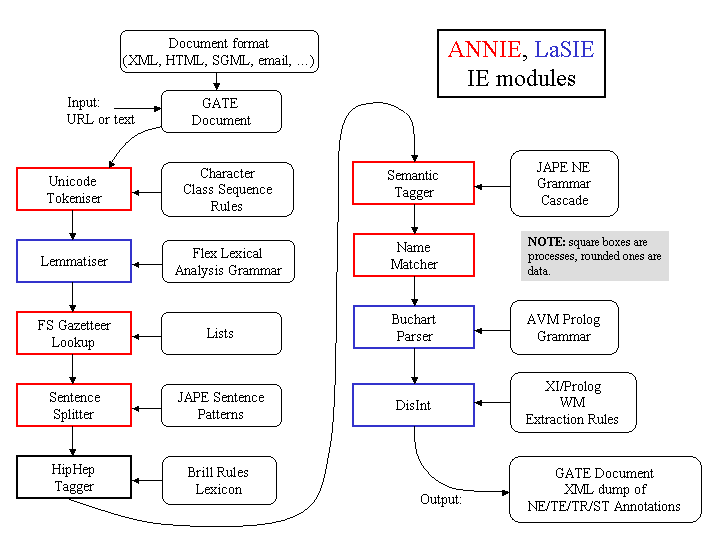
\includegraphics[width=0.8\columnwidth]{img/annie-pipe.png}
    \caption{Classical NLP Pipeline as applied in ANNIE and LaSIE text processing tools}
    \label{fig:nlpipe}
\end{figure}

ATHENA's pipeline is similar in the sense that it prepares the document set during the Harvesting step, then it Enhances the dataset with useful data. The third pipeline step is normalising (or flattening) the data set to its most useful and representative core, while the final step takes as input the normalised document sets and runs a comparative Analysis.

\section{Data modeling and extraction approaches}
The vast domain of text feature extraction and text mining is a very diverse one. A variety of approaches can be applied, as discovered by many branches of research. One of the most important issues to discuss is the advantages and drawbacks of the domain-related and domain-independent categories of machine learning, and what they mean for natural text processing. Towards the end of this section, the discussion will move to scientifically sound and time-proven methods which achieve parts of the necessary functionalities in ATHENA.

\subsection{Supervised vs. unsupervised learning. Domain vs Domain-independent approaches}
As previously discussed, one of the biggest discussions to be had at the start of a text processing application's development, is whether the application will fall into either one of the categories: supervised vs. unsupervised machine learning, domain-related or domain-independent. Usually the categories are coupled in the sense that domain-independent data can not be correctly processed within a supervised approach, which means the two are incompatible.

Supervised learning starts from the premise that we can classify some existing, annotated data, and once the classifier is correctly trained, it can be launched onto the real, full-scale dataset and perform well. Indeed with supervised learning, considering the domain-related approach, an impressive accuracy rate can be obtained. Factors such as the training set size, completeness and correctness influence, along with domain-specific tweaks, can combine to create a powerful classifier. However, there are some drawbacks: 

\begin{itemize}
\item the approach can not be generalised to other domains without existing annotated data for those domains
\item the training set is often difficult to find  and/or manually annotate. Such a training set requires a lot of resources and a dedicated staff, while for the best final accuracy the number of documents correctly labeled in the training set should be very large.
\end{itemize}

Applications such as ATHENA seem to not have a choice but use the domain-independent approach, with specifically domain-independent algorithms to build the analysis results. But the results in the field are not discouraging. In 2002, a study by Turney \cite{turney2002thumbs} found an accuracy rate of 74\% for an unsupervised learning approach, applied to text processing and sentiment analysis in particular. ATHENA does not restrict limits on the hashtags users can use to build harvests, and is in the impossibility of building training sets for all such hashtags, so it falls into the area of unsupervised learning. It is important to note that subsequent algorithms for calculating various application analysis results should therefore also be unsupervised ones.

\subsection{Clustering}
One of the most important unsupervised learning concepts that ATHENA uses, both in the Enhancement and Analysis steps, is that of clustering. Clustering is the grouping of related document features and/or documents, based on common features. It does not require any training data as input and does not have specific domain applicability, which means it is safe to use throughout our application.

A Google Scholar search of the terms "document clustering" produces almost 1.5 million results in books, papers and conference proceedings. The prevalence of clustering algorithms is due to it's easy to understand process and applicability over a large range of possible datasets. A 2000 study by Steinbach et. al \cite{steinbach2000comparison} compares the accuracy of some clustering algorithms, including:

\begin{itemize}
\item K-Means
\item bisecting K-Means
\item UPGMA (Unweighted Pair Group Method with Arithmetic Mean)
\end{itemize}

with different centroid calculation methods. It demonstrates that bisecting K-Means performs best for hierarchical clustering, with some dataset particularities constituting exceptions.

\subsubsection{KMeans}
The clustering algorithm used in ATHENA is K-Means. Initially proposed by Stuart Lloyd in 1957 and applied to research in pulse-code modulation\footnote{https://en.wikipedia.org/wiki/K-means\_clustering}, K-Means has become popular in cluster analysis and data mining after its republication in Fortran by Hartigan and Wong in 1975/1979, which featured better efficiency. The algorithm starts from a number of K centroids and then alternates between two types of steps:

\begin{itemize}
\item assignment: assign each data point to the nearest centroid (in Euclidean distance)
\item update: calculate new centroids at the mean of points assigned to each centroid
\end{itemize}

KMeans runs these steps alternatively until convergence, which is achieved when centroids no longer move from iteration to iteration, or at least do not move over a distance greater than a predefined minimum. In Chapter 4 I will refer to the NP-hard problem of centroid initialisation for encouraging fast convergence, which is based on a 2013 Celebi et. al study \cite{celebi2013comparative} which compares the performance of different centroid seeding methods.

ATHENA uses a variant of KMeans which translates the term occurrence and frequency in the document set to Euclidean distance, i.e. the presence of common terms inside a pair of documents defines the closeness of those documents.

\subsection{Power law dataset analysis}
Another important issue we need to correctly handle is the modelling of users behaviour in authoring documents. We are mostly interested in the degree of fitting of post numbers per user to the existence of a power law. Perhaps one of the best-known example of a power law in effect is that proposed by the Italian economist Vilfredo Pareto, that 80\% of the land in Italy was owned by 20\% of the population. The extension to other fields soon became apparent, with Pareto's law being generalised as: "For many events, roughly 80\% of the effects come from 20\% of the causes\footnote{https://en.wikipedia.org/wiki/Pareto\_principle}. When applying Pareto's law to our dataset of document numbers, it might be the case that unusually high numbers of documents are authored by unusually low numbers of users.

In Nassim Nicolas Taleb's 2007 book "The Black Swan"\cite{taleb2007black}, the principles of power laws are given great focus. The author maintains that the existence of power laws in economic contexts is of such nature, that the modeling of economic events in Gaussian distributions is entirely wrong, with Mandelbrotian (fractal) modeling being far more suitable. The argument is that, in such datasets, the outliers are so powerful, that they skew the results of an otherwise correct calculation. These long tail measures apply mostly to data which is not a physical property such as height or weight of people, but to economic and social aspects such as popularity, wealth, career-wise success. It is probably safe to admit that post numbers and post popularity in social media fall into the same non-physical category which can many a times be modeled as a power law distribution.

As to calculation methods of this fitting degree, authors Clauset et. al built a Matlab implementation of an algorithm doing these estimations. The formal proof of algorithm correctness, as well as arguments for the algorithm, are collected in a 2009 study \cite{clauset2009power}. The same algorithmic approach was later translated to various programming languages either by the authors themselves, or by third party developers interested in using the library. These endeavours saw R, Python, C++ and Java libraries created on the same basic ideas.

\subsection*{Summary}
In this chapter I discussed the similarities between the proposed application of ATHENA and other scientific endeavours to create feature extraction systems. The subjects covered started with arguments for designing ATHENA as a web application and using the pipeline architecture, as validated and widely-used throughout the scientific community concerned with text processing.

I then discussed the advantages and drawbacks of domain-related vs. domain-independent text processing, as well as the supervised and unsupervised approaches, motivating why only the latter is suitable for the ATHENA application and explaining the consequences of this categorisation. In the last part of this section, I covered a couple of algorithms used in the analysis the application performs, with KMeans and Plfit as algorithms suitable to unsupervised learning and thoroughly researched and validated by the scientific community.

More in-depth analysis of existing approaches, their suitability to this project and particular implementations needed will be discussed in the next chapter